% -*- latex -*-

\documentclass{article}

\usepackage{amsfonts}
\usepackage{amssymb}
\usepackage{amsmath}
\usepackage{graphicx}
\usepackage{varioref}
\usepackage{fancyvrb}
\usepackage{ifthen}
\usepackage{cite}
\usepackage{xspace}
\usepackage{hyperref}

\usepackage{color}
\definecolor{yellow}{rgb}{1,1,0}
\definecolor{black}{rgb}{0,0,0}
\definecolor{ltcyan}{rgb}{.75,1,1}
\definecolor{blue}{rgb}{0,0,1}
\definecolor{red}{rgb}{1,0,0}
\definecolor{darkred}{rgb}{0.5,0,0}
\definecolor{darkgreen}{rgb}{0,0.5,0}

% Cite commands I use to abstract away the different ways to reference an
% entry in the bibliography (superscripts, numbers, dates, or author
% abbreviations).  \scite is a short cite that is used immediately after
% when the authors are mentioned.  \lcite is a full citation that is used
% anywhere.  Both should be used right next to the text being cited without
% any spacing.
\newcommand*{\lcite}[1]{~\cite{#1}}
\newcommand*{\scite}[1]{~\cite{#1}}

\newcommand*{\keyterm}[1]{\emph{#1}}

\newcommand{\etal}{et al.}

\newcommand{\fix}[1]{{\color{red}\textbf{\textsc{[#1]}}}}

% Avoid putting figures on their own page.
\renewcommand{\textfraction}{0.05}
\renewcommand{\topfraction}{0.95}
\renewcommand{\bottomfraction}{0.5}

% Make sure this is big enough so that only big figures end up on their own
% page but small enough so that if a figure does have to be on its own
% page, it won't push everything to the bottom because it's not big enough
% to have its own page.
\renewcommand{\floatpagefraction}{.75}

\title{Modern Visualization Pipelines}

\author{Kenneth Moreland}

\date{}

\sloppy

\begin{document}

\maketitle


\section*{Abstract}

The most common abstraction used by visualization libraries and
applications today is what is known as the visualization pipeline.  The
visualization pipeline provides a mechanism to encapsulate algorithms and
then couple them together in a variety of ways.  The visualization pipeline
has been in existence for over twenty years, and over this time many
variations and improvements have been proposed.  This paper provides a
literature review of the most prevalent features of visualization pipelines
and some of the most recent research directions.


\section{Introduction}
\label{sec:Introduction}

The field of scientific visualization was launched with the 1987 National
Science Foundation Visualization in Scientific Computing workshop
report\lcite{ViSC1987}, and some of the first proposed frameworks used a
\keyterm{visualization pipeline} for managing the ingestion,
transformation, display, and recording of
data\lcite{Haeberli1988,Lucas1992}.  The combination of simplicity and
power makes the visualization pipeline still the most prevalent metaphor
encountered today.

The visualization pipeline provides the key
structure in many visualization development systems such as the
Visualization Toolkit (VTK)\lcite{VTK}, SCIRun\lcite{SCIRun}, the
Application Visualization System (AVS)\lcite{AVS}, OpenDX\lcite{OpenDX},
and Iris Explorer\lcite{IRISExplorer}.  Visualization applications like
ParaView\lcite{ParaView}, VisTrails\lcite{VisTrails}, and
MayaVi\lcite{MayaVi} allow end users to build visualization pipelines with
graphical user interface representations.  The visualization pipeline is
also used internally in a number of other applications including
VisIt\lcite{VisIt}, VolView\lcite{VolView}, OsiriX\lcite{OsiriX}, 3D
Slicer\lcite{3DSlicer}, and BioImageXD\lcite{BioImageXD}.

In this paper we review the visualization pipeline.  We begin with a basic
description of what the visualization pipeline is and then move to
advancements introduced over the years and current research.


\section{Basic Visualization Pipelines}
\label{sec:BasicVisualizationPipelines}

A visualization pipeline encapsulates an algorithm in one of three types of
objects: \keyterm{sources}, \keyterm{filters}, and \keyterm{sinks}.  A
source object produces data that it makes available through an
\keyterm{output}.  File readers and synthetic data generators are typical
source objects.  A sink object accepts data through an \keyterm{input} and
performs an operation with no further result (as far as the pipeline is
concerned).  Typical sinks are file writers and rendering components that
provide images to a user interface.  A filter object has at least one input
from which it transform data and provides results through at least one
output.

The intention is to encapsulate algorithms in interchangeable source,
filter, and sink components with generic connection ports (inputs and
outputs).  An output from one component can be connected to the input from
another component such that the results of one algorithm become the inputs
to another algorithm.  These connected components form a
\keyterm{pipeline}.  Figure~\ref{fig:SimplePipeline} demonstrates a simple
but common pipeline featuring a file reader (source), an isosurface
generator\lcite{Lorensen1987} (filter), and an image renderer (sink).

\begin{figure}[htbp]
  \centering
  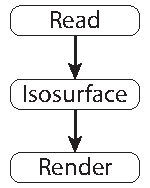
\includegraphics{images/SimplePipeline}
  \caption{A simple visualization pipeline.}
  \label{fig:SimplePipeline}
\end{figure}

Pipeline components are highly interchangeable.  Any two components can be
connected so long as the data in the output is compatible with the expected
data of the downstream input.  Pipelines can be arbitrarily deep.
Pipelines can also branch.  A \keyterm{fan out} occurs when the output of
one component is connected to the inputs of multiple other components.  A
\keyterm{fan in} occurs when a component accepts multiple inputs that can
come from separate component outputs.  Figure~\ref{fig:BranchingPipeline}
demonstrates a pipeline with branching (adapted from the ParaView
tutorial\lcite{ParaViewTutorial}).

\begin{figure}[htbp]
  \centering
  \begin{tabular}{cc}
    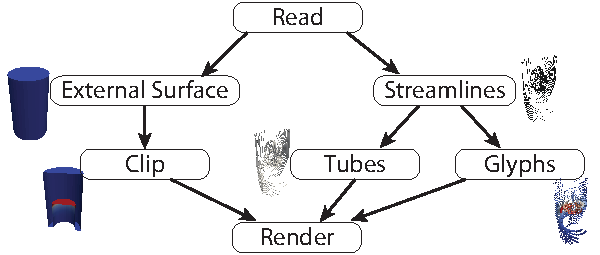
\includegraphics{images/BranchingPipeline} &
    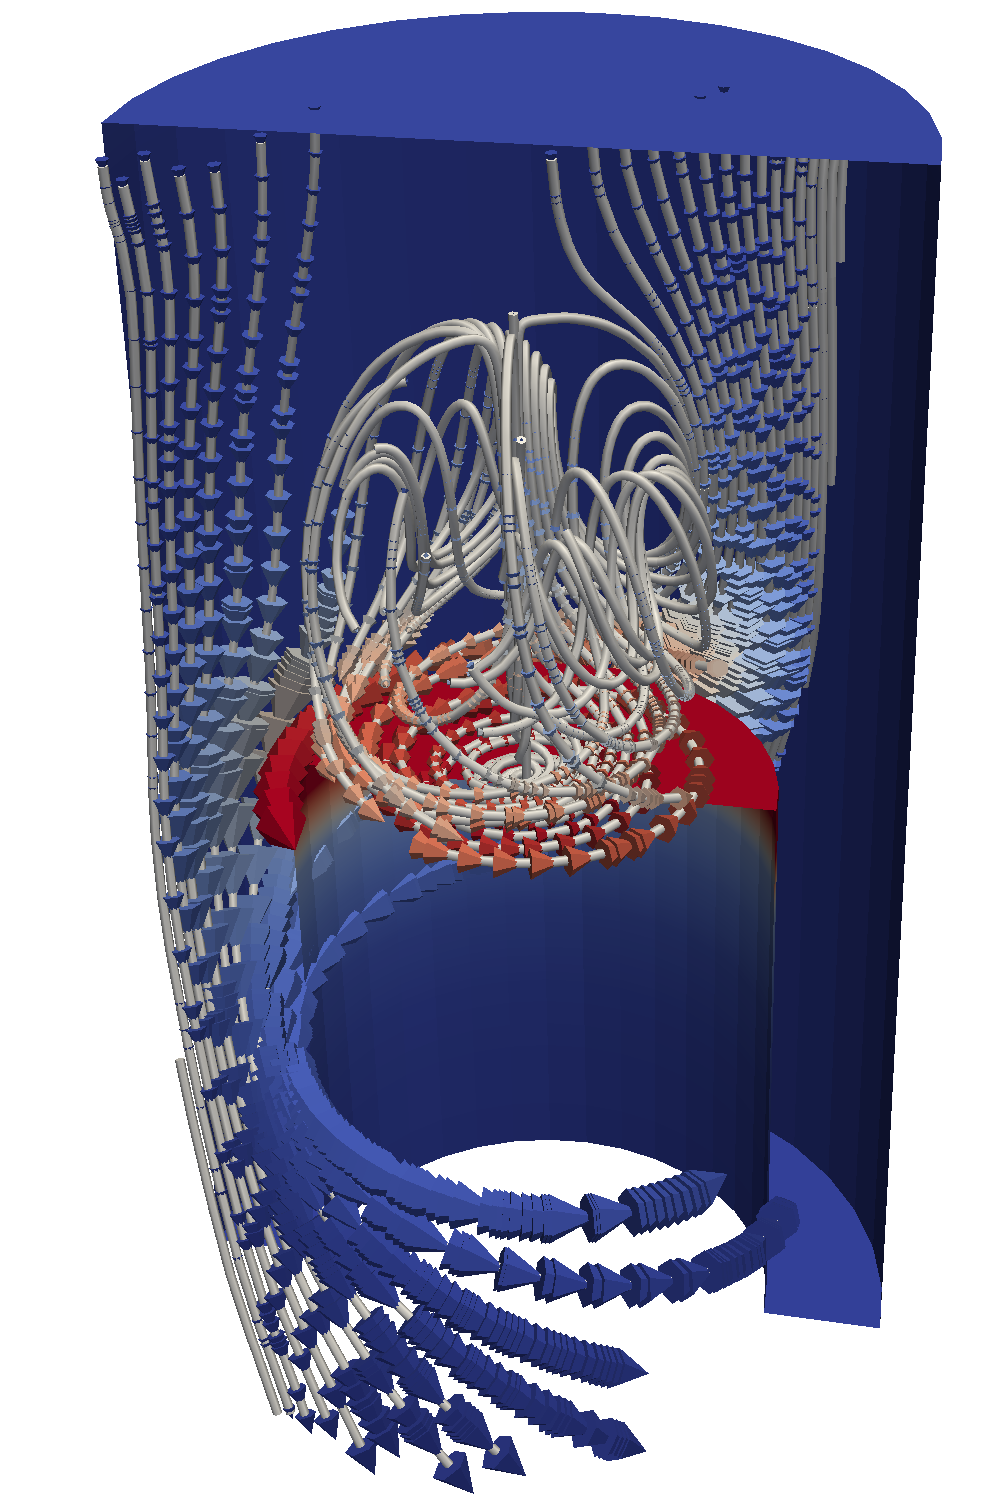
\includegraphics[height=1.7in]{images/BranchingPipelineResult}
  \end{tabular}
  \caption{A visualization pipeline with branching.  The final
    visualization is shown to the right.}
  \label{fig:BranchingPipeline}
\end{figure}

For more information on using visualization pipelines and the components
they typically contain, consult the documentation for one of the numerous
libraries or applications using a visualization
pipeline\lcite{VTK,ParaView,ParaViewTutorial,SCIRunUserGuide,IRISExplorerUsersGuide}.
\fix{Add OpenDX.  Site was down.}


\section{Execution Management}
\label{sec:ExecutionManagement}

\subsection{Push vs. Pull}
\label{sec:PushPull}

\subsection{Centralized vs. Distributed}
\label{sec:CentralizedDistributed}

\subsection{Block Iteration}
\label{sec:BlockIteration}

\subsection{Detached Executive}
\label{sec:DetachedExecutive}


\section{Metadata}
\label{sec:Metadata}

\subsection{Extents}
\label{sec:Extents}

Reporting extents in multiple passes.

Sending extent requests up pipeline.

\subsection{Contracts}
\label{sec:Contracts}

\subsection{Time}
\label{sec:Time}

\subsection{Prioritized Streaming}
\label{sec:PrioritizedStreaming}

\subsection{Query Driven Visualization}
\label{sec:QueryDrivenVisualization}


\section{Parallel Execution}
\label{sec:ParallelExecution}

\subsection{Basic Parallel Execution Modes}
\label{sec:ParallelExecution:Modes}

\subsection{Rendering}
\label{sec:ParallelExecution:Rendering}

\subsection{Scalability}
\label{sec:Scalability}

\subsection{Hybrid Parallel}
\label{sec:HybridParallel}


\section{Miscellany}
\label{sec:Misc}

\subsection{Provenance}
\label{sec:Provenance}

\subsection{Scheduling}
\label{sec:Scheduling}

Multi-core.  Heterogeneous.  Hyperflow.

\subsection{In Situ}
\label{sec:InSitu}


\section{Visualization Pipeline Alternatives}
\label{sec:Alternatives}

\subsection{Field Abstraction}
\label{sec:FieldAbstraction}

Field Model (FM).  Field Encapsulation Library (FEL).

\subsection{MapReduce}
\label{sec:MapReduce}

\subsection{Worklets}
\label{sec:Worklets}


\section{Conclusion}
\label{sec:Conclusion}


\section{Acknowledgments}

This work was supported in part by the DOE Office of Science, Advanced
Scientific Computing Research, under award number 10-014707, program
manager Lucy Nowell.

Sandia National Laboratories is a multi-program laboratory operated by
Sandia Corporation, a wholly owned subsidiary of Lockheed Martin
Corporation, for the U.S. Department of Energy's National Nuclear Security
Administration.

\bibliographystyle{plain}
\bibliography{VisPipelines}

\end{document}
